\section{Campionamento}
Il campionamento è un processo che legge valori distanziati l'uno dall'altro con un passo $\Delta t$ approssimato al tempo infinitesimo, ma in realtà discreto. La scelta dell'ampiezza del passo deve evitare sia lo spreco di risorse che la perdita di informazioni.

Il segnale, in pratica, passa dall'analogico al digitale e dal continuo al discreto, e viene rappresentato come una serie di impulsi.

A una funzione campionata (con passo $\Delta x$) corrisponde nel dominio trasformato uno spettro periodico. Il periodo è inversamente proporzionale al passo di campionamento (ricostruzione della funzione continua dalla trasformata).

Così come a una funzione continua nel dominio dello spazio ne corrisponde una nel dominio delle frequenze espressa come somma pesata di armoniche (analisi e sintesi), a una funzione campionata con passo $\Delta x$ corrisponde nel dominio trasformato uno spettro periodico, con periodo in funzione del passo di campionamento.
$$F(u) = \sum_{k=-\infty}^{\infty} f(k\Delta x)e^{-j2\pi uk \Delta x}$$
La frequenza di campionamento minima, quindi, garantisce un periodo sufficientemente grande per contenere l'intero spettro. Esso è simmetrico, quindi $-f_{max} = f_{max}$ come visto nel dominio della trasformata di Fourier.

Se il passo di campionamento è troppo alto ($\Delta x' = 1/M > \Delta x = 1/N$), le repliche dello spettro si sovrappongono (periodo $M$ troppo breve) e non è possibile risalire alla funzione originale. \\
Questo succede perché le alte frequenze che non vengono considerate (a causa dell'alta variabilità del segnale, che non può essere interpretata in un periodo) ma si sovrappongono alle più basse, causando una errata rappresentazione.

Al contrario, una bassa frequenza di campionamento produce fenomeni di aliasing: la funzione viene approssimata male, come costante o una differente sinusoide.

Il teorema di Shannon afferma che, data la frequenza massima del segnale $f_{MAX}$, la frequenza massima di campionamento deve essere:
$$F_s = \nicefrac{1}{\Delta} > 2f_{MAX}$$
Il periodo minimo di ripetizione dello spettro perché non vi sia sovrapposizione $N = 2f_{MAX}$. La $f_{MAX}$ viene definita frequenza di Nyquist, e rappresenta la frequenza massima del segnale.

Lo spazio pertanto sarà $2f_{MAX}$, il che è il minimo valore per evitare le sovrapposizioni delle repliche. Nella formula viene utilizzata la disuguaglianza stretta per assicurare che non ci siano due frequenze nello stesso punto.

Per eliminare le frequenze alte e di conseguenza ridurre il passo di campionamento si ricorre al filtraggio (filtro anti-aliasing), che comunque non assicura il recupero della funzione originale ma evita le sovrapposizioni.

L'aliasing è appunto il fenomeno per cui il segnale originale non è ricostruibile dato che il campionamento è avvenuto con frequenza inferiore a quella di Nyquist, e il segnale risultante ha frequenza inferiore all'originale. Questo può gravemente compromettere la qualità di immagini e video: nella pratica i segnali non sono limitati in frequenze, ma nel tempo, quindi le repliche di uno spettro vanno separate attentamente tramite filtri passa-basso.

Quando il segnale è campionato, la variabile tempo/spazio non è più esplicita e la frequenza $f_N$ rappresenta il numero di cicli per campione.

\subsection{Esempio}
$$x(n) = A\cos(\omega n + \theta)$$
\begin{figure}[h]
	\centering
	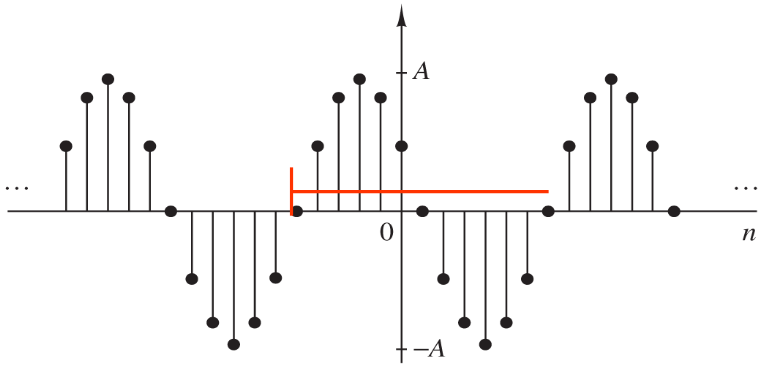
\includegraphics[scale=0.56]{Lezioni/Immagini/esempio1}
\end{figure}

$\omega = 2\pi f_N$, dove $\omega$ è la pulsazione e $f_N$ la frequenza normalizzata, cioè il numero di cicli al secondo (continuo), con campioni al posto dei secondi nel mondo campionato.

Per capire la frequenza $f_N$ del segnale rappresentato, bisogna guardare quanti cicli ci sono per campioni (o quanti campioni ci sono in un ciclo, cioè prima che il pattern si ripeta) e calcolare l'inverso. In questo caso un periodo è 12 campioni, quindi $f_N = 1/12$.

La frequenza al secondo (Hz) è ottenibile sapendo quanta distanza c'è tra un campione e l'altro, altrimenti per ogni rappresentazione ci sarebbero infinite sinusoidi.

La pulsazione $\omega$ è uguale a $2\pi f_N$, quindi $\frac{2\pi}{12} = \frac{\pi}{6}$. \\
Lo sfasamento con anticipo di 2 campioni si trova effettuando la proporzione: un periodo è $2\pi$, se 12 campioni sono in$2\pi$ allora $2\pi : 12 = \theta : 2 \rightarrow \theta = \frac{\pi}{3}$.

La frequenza normalizzata indica quanto bene si vedono i campioni e la loro variazione in un periodo, per poi decidere la finestra di osservazione. La frequenza dipende dal numero di campioni al secondo ($f_c$): se la frequenza di campionamento è $f_c = 1$ campione/secondo, si ha che $f = 1/12$ ciclo/secondo, cioè $f = f_c \cdot f_N$.

Per ricavare la formula più facilmente si possono utilizzare le unità di misura. Un altro modo per arrivare allo stesso risultato è sostituire a $n\Delta t$ la $t$.

Con 2 campioni al secondo, cioè $f_c = 2$ e $\Delta t = 0.5 = \nicefrac{1}{2}$, la frequenza $f$ in cicli al secondo (Hz) è $\nicefrac{1}{2}$:
$$f_N \cdot f_c = \frac{1}{12} \frac{\text{cicli}}{\text{campione}} \cdot \frac{2 \text{ campioni}}{\text{sec}} = \frac{1}{6} \frac{\text{cicli}}{\text{sec}}$$
$$x(n) = A\cos \Big(2\pi \frac{1}{12}n + \frac{\pi}{3}\Big) \implies x(t) = A\cos\Big(2\pi \frac{1}{6}t + \frac{\pi}{3}\Big) \qquad \Delta tn \implies t$$

\subsubsection{Frequenze}
Il range tra minimo e massimo di una frequenza di oscillazione è 1, tutto ciò che è al di fuori dell'intervallo in realtà si trova comunque normalizzato all'interno. Aumentando $\omega$, infatti, dopo un giro (periodo $2\pi$) si torna ad avere la stessa funzione. 

Frequenza minima di oscillazione di una sinusoide a tempo discreto: $f_N = 0 \rightarrow \omega = 0$ \\
Frequenza massima di oscillazione di una sinusoide a tempo discreto: $f_N = \pm \nicefrac{1}{2} \rightarrow \omega = \pm \pi$ \\
Frequenza di oscillazione di una sinusoide generica: $f = \frac{1}{\text{n. campioni}} \rightarrow \omega = 2\pi \cdot f_N$

I segnali sinusoidali a tempo discreto con pulsazioni separate da multipli di $2\pi$ sono identici: \\
$\omega + k2\pi = \omega$ con $k \in \mathbb{Z}$ \\
$x(n) = \cos(\omega n + \theta)$ \\
$\cos((\omega + 2k\pi)n + \theta) = \cos(\omega n + \theta)$ \\
$\cos(\omega n + kn2\pi + \theta) = \cos(\omega n + \theta)$

Per convenzione si utilizza la frequenza di Nyquist, $f_n = [-\nicefrac{1}{2}, \nicefrac{1}{2}]$, oppure intervalli di pulsazione $[-\pi, \pi]$ o $[0, 1] \rightarrow [0, 2\pi]$.

Il segnale è periodico solo se la sua frequenza $f$ è un numero razionale: $f = \nicefrac{k}{N}$.



Il segnale sinusoidale è periodico se e solo se la sua frequenza normalizzata $f$ è un numero razionale (rapporto fra due interi). I numeri razionali quindi impongono la periodicità. 
